
% to choose your degree
% please un-comment just one of the following
\documentclass[bsc,frontabs,twoside,singlespacing,parskip,deptreport]{infthesis}     % for BSc, BEng etc.
% \documentclass[minf,frontabs,twoside,singlespacing,parskip,deptreport]{infthesis}  % for MInf
\usepackage{float}
\begin{document}

\title{A Network Extension for the Gamemaker HTML5 Export Module}

\author{Teun Kokke}
\course{Software Engineering} 
\project{Undergraduate Dissertation} % CS&E, E&SE, AI&L

\date{\today}

\abstract{
summarising the report\\
Creating an extention for Gamemaker creations, to allow fast networking with maximal reliability.
}

\maketitle

% REMOVE THESE >>>>
\section*{QUESTIONS TO SUPERVISOR}
\begin{itemize}
\item Need to mention examples in background for "why gamemaker"? if no, where should examples be given if at all?
\item Known from previous experiments: a single instance cannot simulate more than roughly 700 clients without causing losing stability. Do I have to show this in detail with a graph as part of the experiments, or should I just mention that eg. 500 clients per instance is arbitrary for this reason and ignore the details?
\item Is it required to include formulae for mean, variance and standard-deviation?
\item Found tex templates from university on website. Use those, or keep this one?
\end{itemize}

\section*{TODO}
\begin{itemize}
\item give definition for server-reponse time
\item Add abbreviation / terminology legend in preamble, eg TCP, UDP, RTT, CPU time, CPU usage, RSS.
\item in section "fairness depending on location", add world map with tested locations and their average mean
\item Consider actual playability in a game OR add assumption how RTT affects atual usage of an application (find reference?)
\item fill in further details on experiment setup (text format)
\item Write down sections for literature, references
\item Write down details about implementation
\item Possibly add new implementation features / clean up existing implementations.
\item Contact community
\end{itemize}
% <<<< REMOVE THESE

\section*{Acknowledgements}
Acknowledgements go here. 
Found people across the globe to assist in testing, family, friends and people found through social media, the Dutch Gamemaker community and the Yoyogames forums.
\tableofcontents

%\pagenumbering{arabic}

% START THE REAL CONTENT


% -----------------------
\chapter{Background and Related Work}
\section{Background}
%intro and synopsis (topic description and setting context of published literature, main results summarized.. about 5 pages)
%- summary of ALL contributions, code, research interpretations, tests, experiments (bulleted list)
\subsection{HTML5}
\paragraph{}HTML5 was released in 2014 (October 28th) by the World Wide Web Consortium (W3C) and is a raising web standard, improving its predecessor HTML4 with the aim to reduce the dependence of functionality from third-party plugins such as Flash and Java applets, which are deprecated and unsupported by many devices\footnote{http://i-programmer.info/news/86-browsers/8783-death-of-flash-and-java.html}.

Scripting is replaced in HTML5 by markup where-ever possible, causing the world of browser-gaming to change rapidly. One of the the newly introduced features is the <canvas> tag, giving rise to isometric JavaScript applications.

\subsection{NodeJS}
%include socket.io %benchmarks for socket.io made by other developers

NodeJS \footnote{http://www.toptal.com/nodejs/why-the-hell-would-i-use-node-js}
\subsection{GameMaker}
%include its evolution and typical target audience
%explain the types of target audience, who do the developers of an application using the extension intend to target. How does this affect the demands on the network
%focus on location of users
\paragraph{}Gamemaker by YoyoGames is a software creation tool with the aim to simplify and speed up game and app development. It is cheap, simple to learn and flexible to use, making the software demanded by small teams, professionals and novice developers. Consequently, the human nature of staying within trusted environments causes developers to stick to Gamemaker.

During the rise of HTML5 and the growing popularity of Gamemaker, YoyoGames has provided the functionality to export any application to a JavaScript program that can be executed directly in the browser. This way i.a. updates can be made seamless, require no file-download nor installation, is platform-independent and easier to distribute.

Some features are lost during the transition from a windows-executable to a web-application. One of them is a critical component to application popularity: networking functionality. Since the HTML5 update in September 2011, this feature was never added.

The implementation in this Honours project will allow developers to again add networking features to their web-browser applications.

\subsection{Networks in Applications}
%include minimal requirements
%which criteria to consider when testing a network
ref for fairness and playability \cite{Fairness_and_Playability}
ref for multiplayer networking in modern game engines \cite{Multiplayer_Networking_modern_engine}

%minimal requirements for a network for a proper user experience
http://drewww.github.io/socket.io-benchmarking/
\\http://blog.mixu.net/2011/11/22/performance-benchmarking-socket-io-0-8-7-0-7-11-and-0-6-17-and-nodes-native-tcp/
\subsection{TCP and UDP}
\subsection{Inter-application Communication}
%how do applications communicate
%IMPORTANT: State why there is no need for testing fairness between different bandwidths for web applications. (ie. games and web-apps only really need to send small variables, no big data is transported)

\section{Related Work}
\subsection{Unity}
\subsection{Unreal Engine 4}
\subsection{CryEngine}
\subsection{Havok Vision Engine}
\subsection{Project Anarchy}
\subsection{ShiVa}
\subsection{App Game Kit}
\subsection{GameSalad}
\subsection{...}






% -----------------------
\chapter{Literature Review}

\section{Multiplayer Networking in Modern Game Engines}

\section{Fairnesss and Playability in Online Multiplayer Games}

\section{...}





% -----------------------
\chapter{Development}
%discussion of work undertaken, sub-problems, solutions, difficulties
%\\- concentrated discussions for implementation principles and aspects
%\\- clarify WHAT WAS COMPLETED, and what wasnt.
\section{Design}
%about the high level design ideas / structure and templates for other developers, make clear connection with literature review
\subsection{Prior Considerations}
%How to make it easy for other developers to create applications with the extension. eg. Creating templates
%project layout (modularisation / separation of concerns). client, server, benchmark application, equality application, user experience
\subsection{Server and Client}
\subsubsection{Good Coding Practices}
\subsubsection{Interaction}
%Mapping from GML to the extension

\section{Implementation}
\subsection{Server}
\subsection{Client}
\subsection{The Extension}
\section{Applications Developed with the Extension}
%Explain about ownmade application using the extension, how it tests the given benchmarks (eg. delay, data, equality)
\subsection{Benchmark Application}
\subsection{Real Game Application}
\subsection{Developer Template}







% -----------------------
\chapter{Network Extension Evaluation}
%description of experiments, presentation + (directly including) interpretation of the data
\section{Setup}
%explain every detail of how the experiments were setup, how everything worked.
%Note: add reminder that developers can setup peer-to-peer network by using the extension to serve as both server and client in their client application, but that these tests specifically consider the strength of each individual application acting as server.

\subsection{Controlled Network Experiments}
The controlled experiments were conducted in order to predict server behaviour when loaded under similar pressure in future occasions. 

\subsubsection{Concurrent Connections Specifics}
\paragraph{Environment}
\begin{itemize}
\item Variable number of concurrent connections cc, up to 15 instances with each simulating at most 500 clients.
\item Clients do not contact the server after establishing a connection.
\item The CPU usage, time and RSS (Resident set size) are recorded after each every time another group of 100 clients connect to the server.
\end{itemize}
\paragraph{Dependent variables}
\begin{itemize}
\item CPU usage on the server
\item CPU time on the server
\item RSS on the server
\end{itemize}

\subsubsection{Message Broadcasting Specifics}
\paragraph{Environment}
\begin{itemize}
\item 5000 concurrent connections (10 instances each simulating at most 500 clients).
\item Each package that is sent has a size of 8 bytes.
\item Each client sends packages at regular time intervals, causing the server to handle n messages every second.
\item Each client measures the roundtrip time of its package to the server.
\end{itemize}

\paragraph{Dependent variables}
\begin{itemize}
\item Mean roundtrip time between all clients
\item Variance of the roundtrip time between all clients
\item Standard Deviation of the roundtrip time between all clients
\end{itemize}

\subsubsection{Server hardware and network specification}
\paragraph{}The controlled network experiments were executed on a Windows 7 64-bit platform with 12.6GB available physical memory and an Intel(R) Core(TM) i7-2600K CPU @ 3.40GHz processor. The software included Node v0.12.3 and Socket.io v1.3.7 in order to handle the networking operations.

The network was controlled using Dummynet, using a below-average UK household network setup. This involves an upload speed of 5Mbit/s, and a download speed of 1Mbit/, although no packet loss was set in order to ensure consistency throughout the controlled network experiments.

\subsection{Real Network Experiments}
The network was consistently running with a 54.0Mb/s download and 3.0Mb/s upload speed.
\paragraph{}All network experiments are executed on a single server located in Edinburgh. In each experiment all clients were connected and communicating to the server simultaneously.



\section{Results}
\subsection{Controlled Network Results}
\subsubsection{Concurrent Connections}
The following experiment evaluates the server performance with regard to the number of clients.

\begin{center}
\begin{figure}[H]
\label{fig:cpu_usage}
% \centering% default with `floatrow`
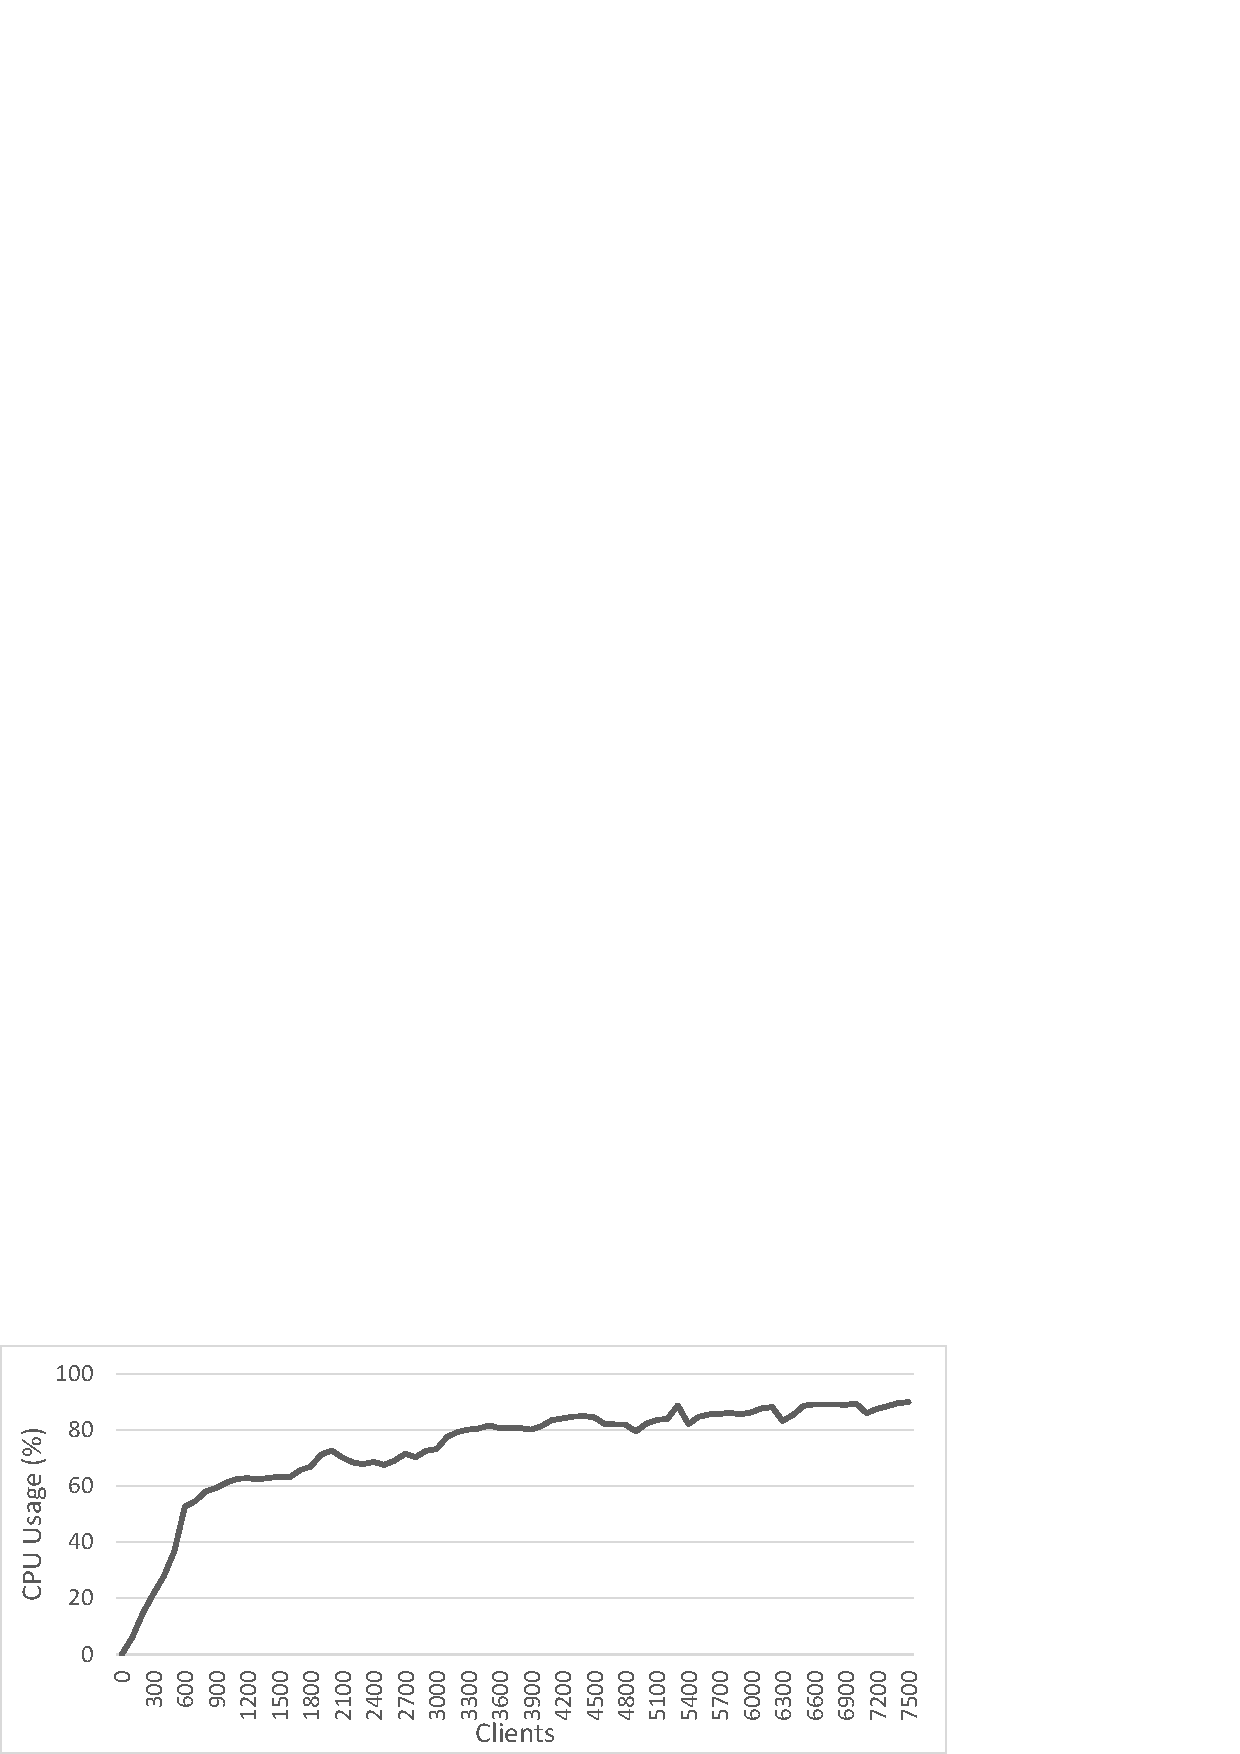
\includegraphics[scale=0.75]{images/test_CLIENT_CPUusage.jpg}
\caption{Displaying the CPU usage for the server process in percent.}
\vspace{1em}
When the CPU usage is above 70 percent, the user may experience lag. Such high CPU usage indicates insufficient processing power. Either the CPU needs to be upgraded, or the user experience reduced.
\end{figure}

\begin{figure}
\label{fig:cpu_time}
% \centering% default with `floatrow`
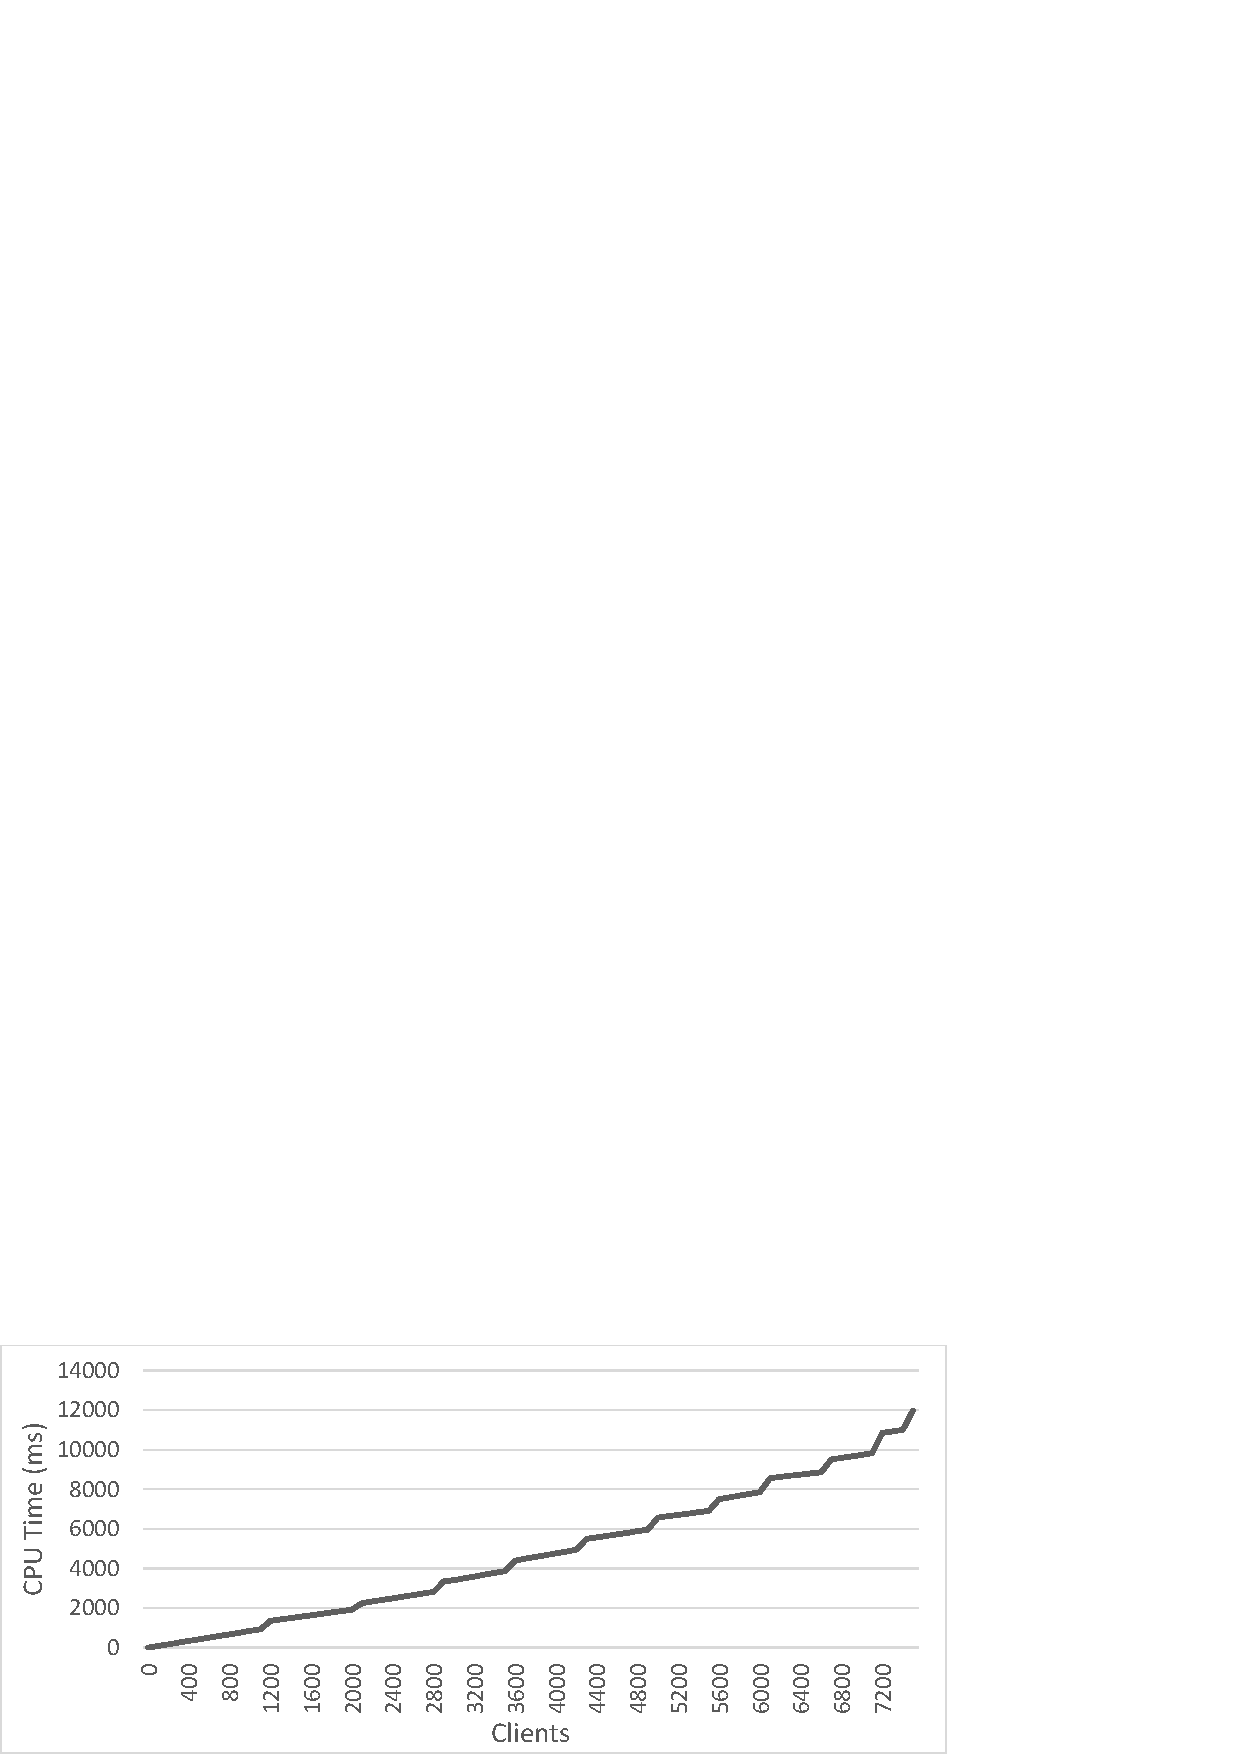
\includegraphics[scale=0.75]{images/test_CLIENT_CPUtime.jpg}
\caption{CPU time in milliseconds, displaying the amount of time required for the server to process the clients.}
\end{figure}

\begin{figure}
\label{fig:cpu_rss}
% \centering% default with `floatrow`
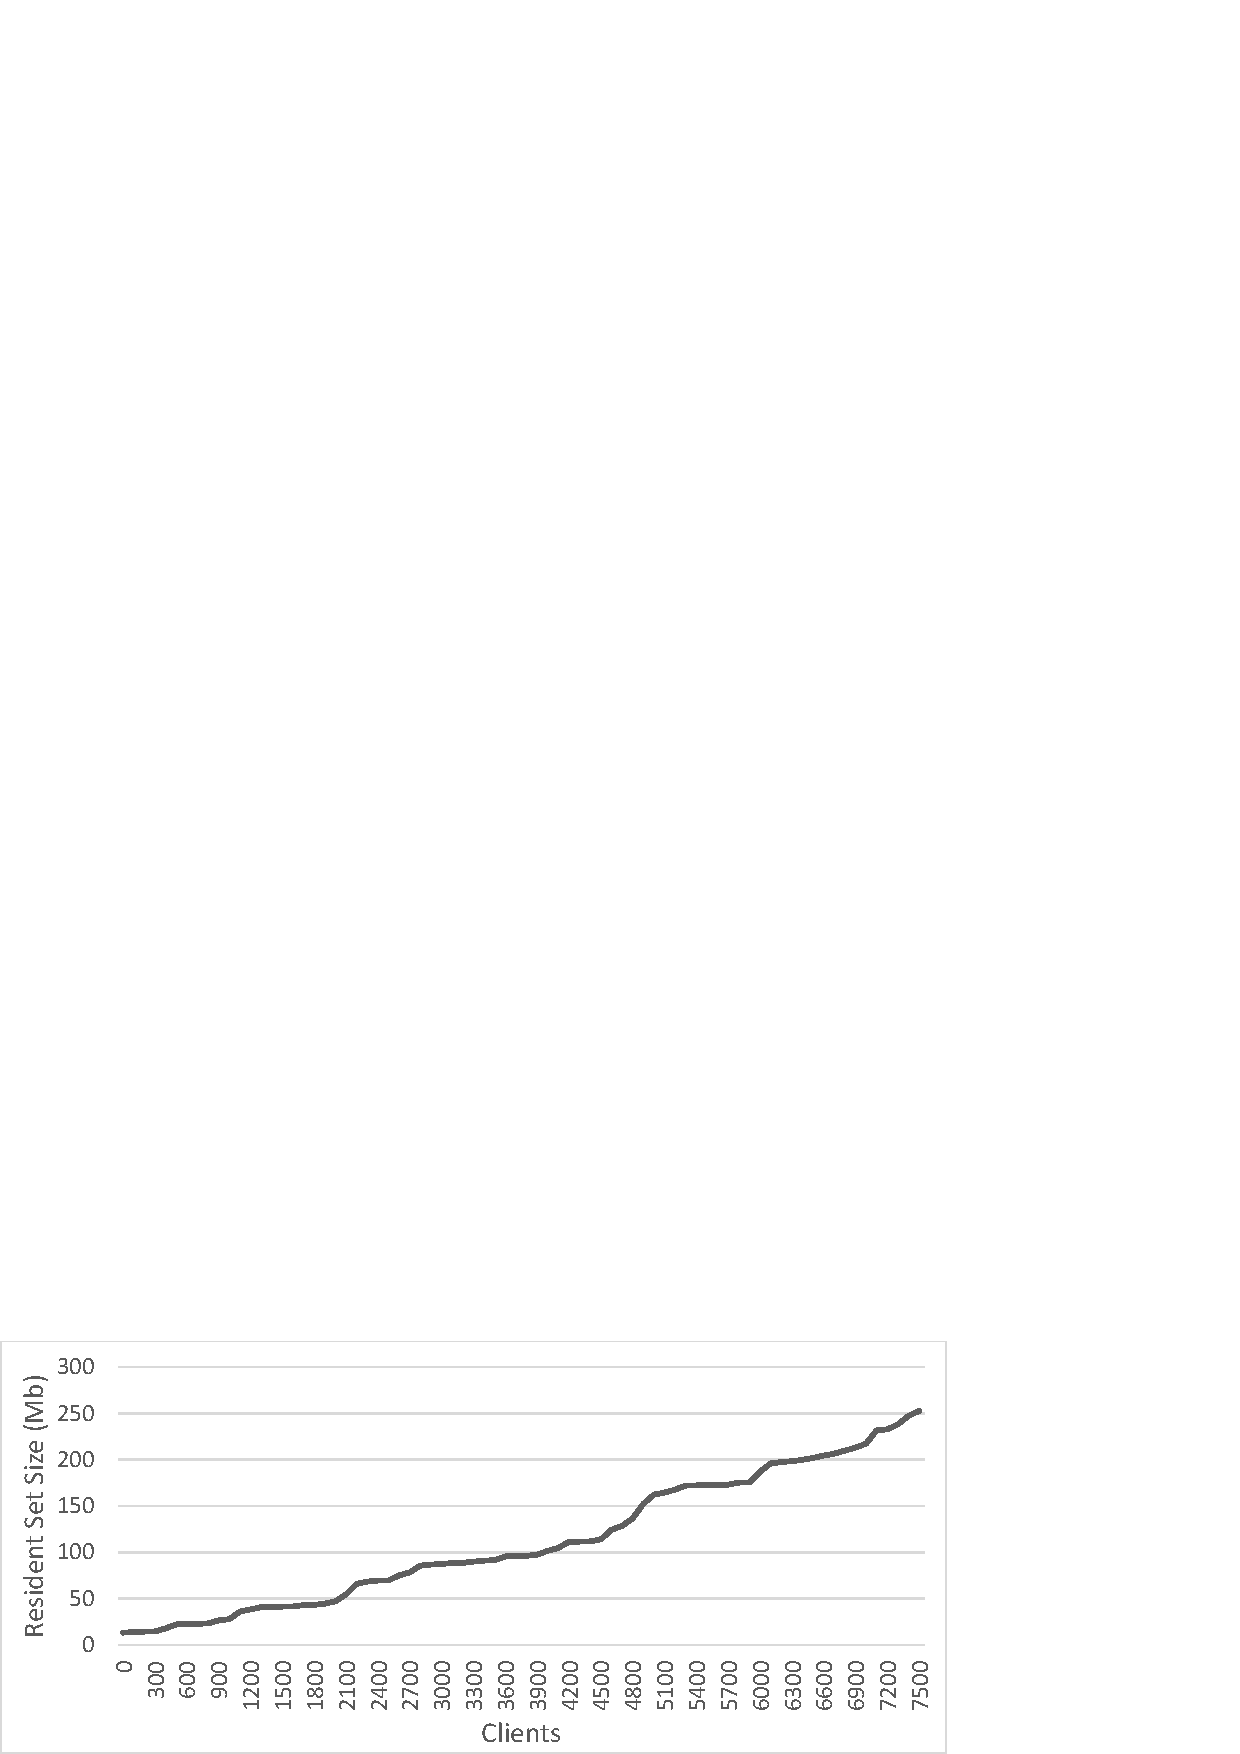
\includegraphics[scale=0.75]{images/test_CLIENT_RSS.jpg}
\caption{Resident set size in Megabit, showing the portion of RAM that is occupied by the server process.}
\end{figure}

\end{center}


\subsubsection{Message Broadcasting Performance}
The following experiment evaluates the number of messages that can be handled by the server simultaneously, and considers how this affects the fairness in response-time of the individual clients.

\begin{center}

\begin{figure}[h]
\label{fig:broadcast_rtt_mean}
% \centering% default with `floatrow`
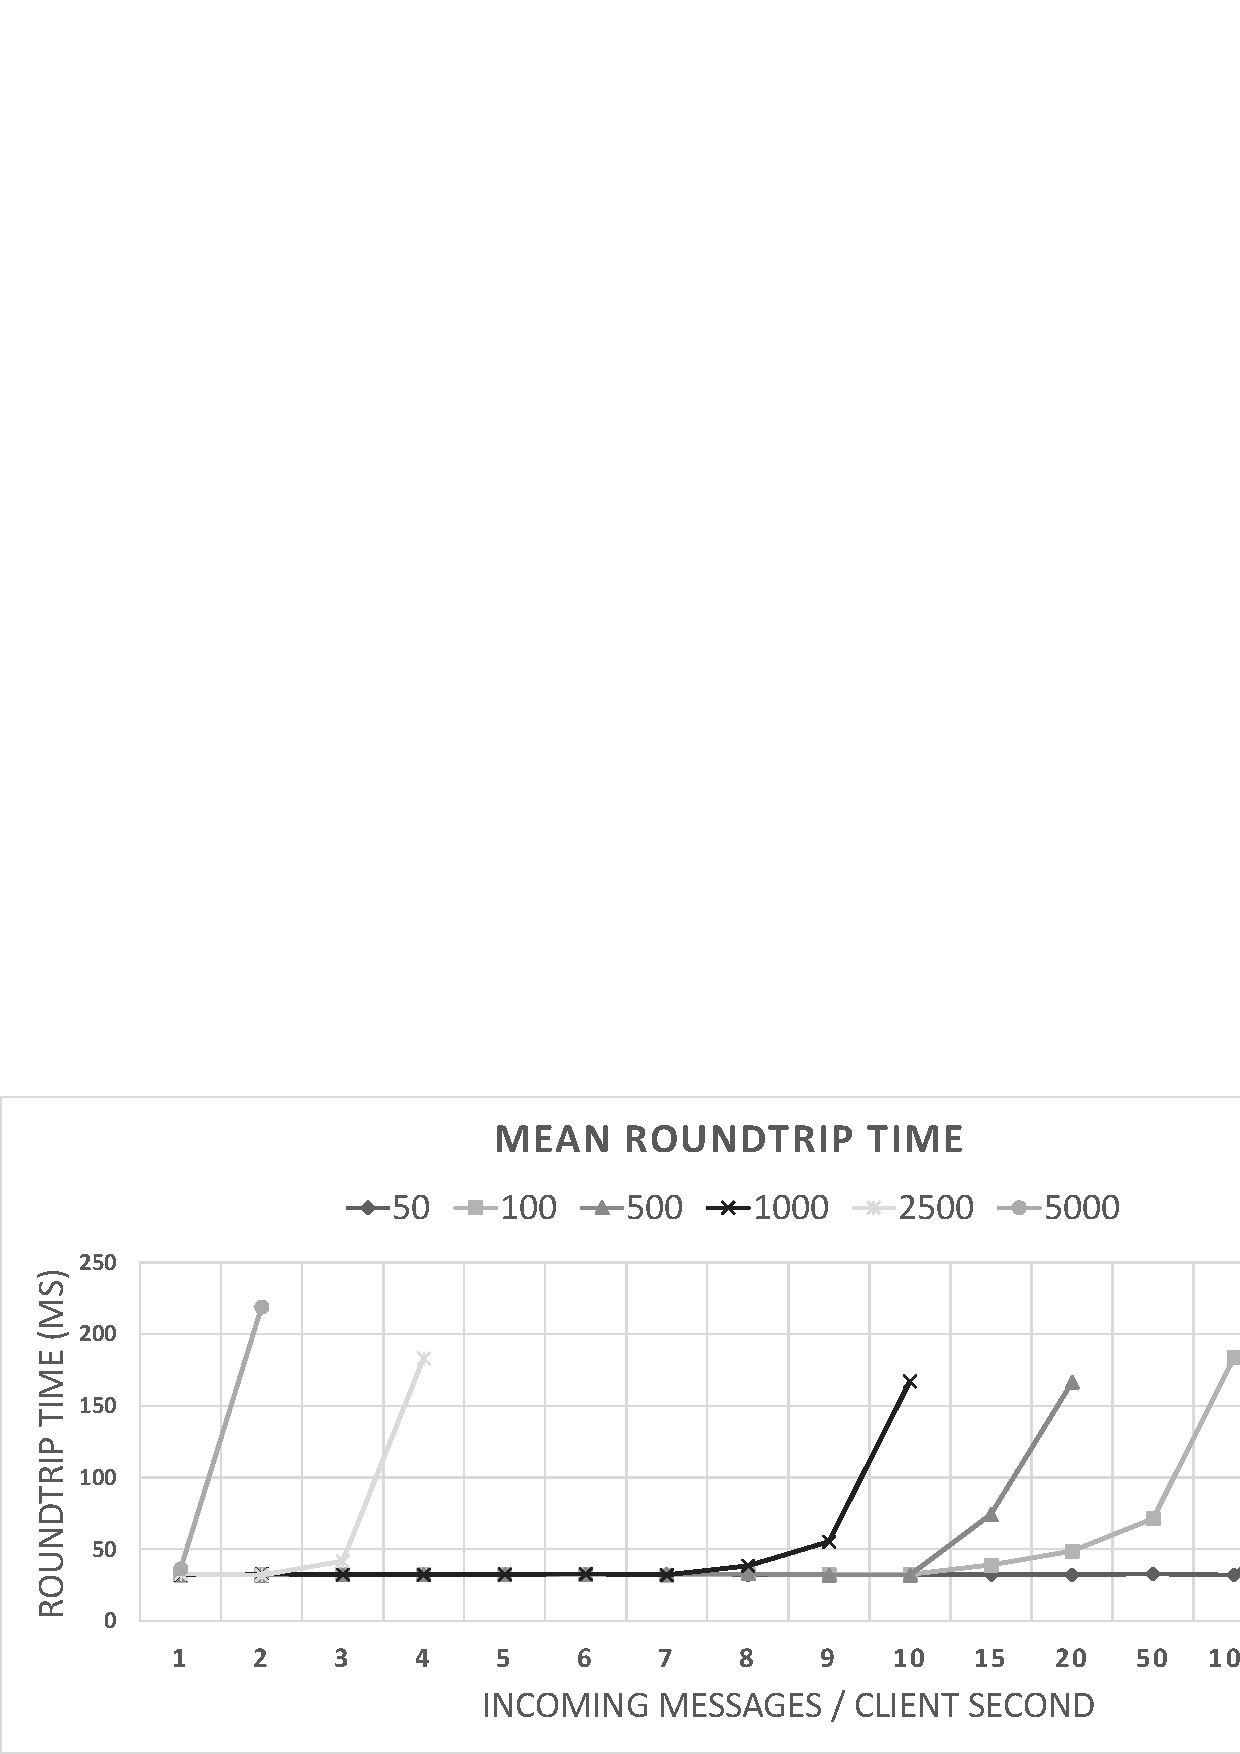
\includegraphics[scale=0.32]{images/test_SERVER_RTTmean.jpg}
\caption{The mean roundtrip time of all the messages that pass through the server. As expected, with few concurrent clients connected to the server, the server manages to broadcast many more messages.}
\end{figure}


\begin{figure}
\label{fig:broadcast_rtt_variance}
% \centering% default with `floatrow`
\includegraphics[scale=0.32]{images/test_SERVER_RTTvariance.jpg}
\caption{The variance of the roundtrip times, showing the fairness between clients decreases significantly when the server receives messages faster than it can broadcast.}
\end{figure}


\begin{figure}
\label{fig:broadcast_rtt_std}
% \centering% default with `floatrow`
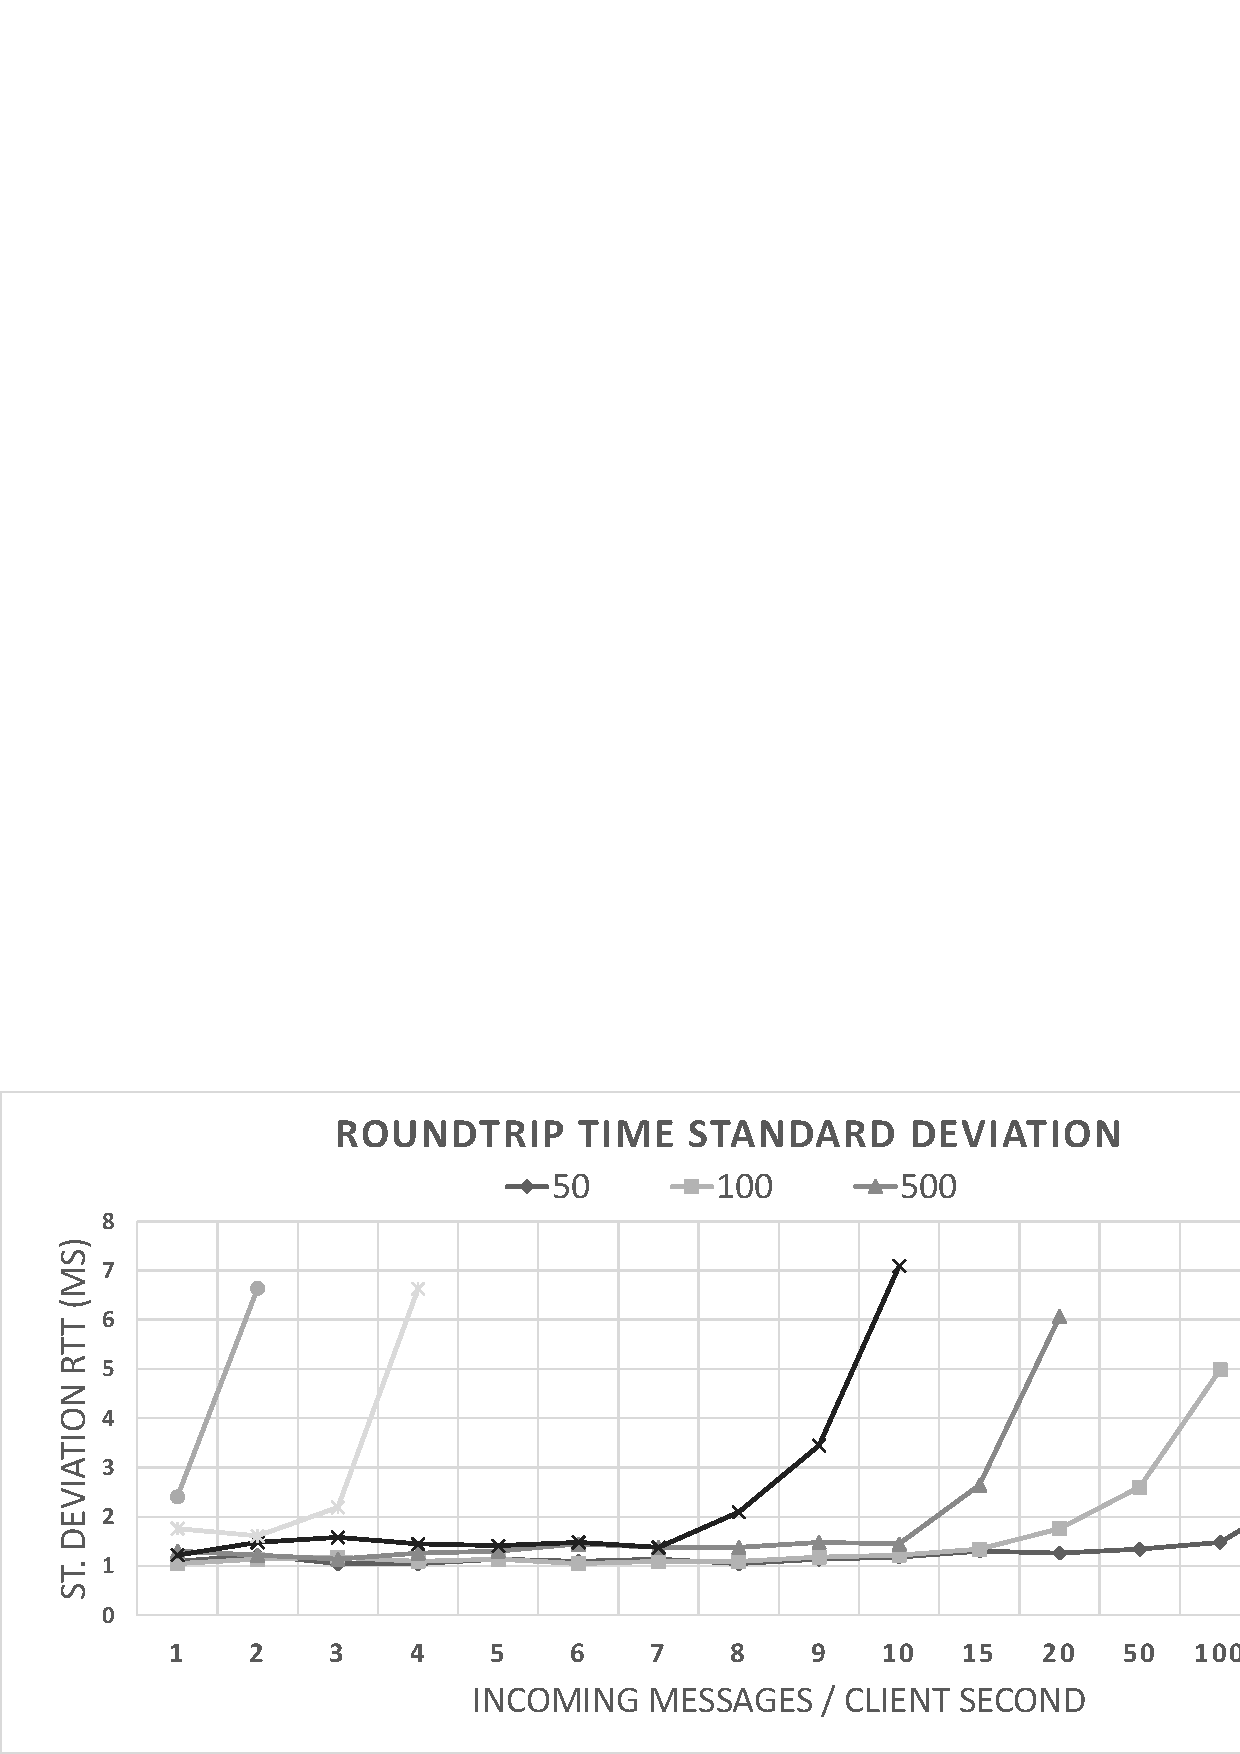
\includegraphics[scale=0.32]{images/test_SERVER_RTTstd.jpg}
\caption{Standard deviation of the message roundtrip times.}
\end{figure}

\end{center}



\subsection{Real Network Results}
\subsubsection{Location-wise Delay Fairness}
The following experiment evaluates the effect of the geographical distance between groups of clients and the server with respect to fairness in response-time from the server to the clients.





% -----------------------
\chapter{Conclusion and Future Work}
\section{Conclusion}
\subsection{Comparison of the Extended GameMaker Functionality with Related Work}
\subsection{Criticism on the Implementation and Design Decisions}
%make clear connection with the evaluation

\section{Future Improvements}






% -----------------------
% use the following and \cite{} as above if you use BibTeX
% otherwise generate bibtem entries
\bibliographystyle{plain}
\bibliography{mybibfile}

\end{document}
